\chapter{Enhanced 8-point and 5-point reconstruction}\label{chap:enh_5_8_point}
\section{Concept} % top level followed by section, subsection
As indicated in a similar research (Chapter 3), it is very attractive to use additional data to enhance reconstruction and reduce ambiguity in finding correct solution for 3D reconstruction. Additional camera or model information help to implement faster, more stable and robust algorithms. This thesis will show how the prior knowledge of rotation or translation acquired via mobile sensor fusion can be used to enhance process of 3D reconstruction from a series of images. When it comes to relying on hand-held smartphones, the collected sensor data are very noisy. This thesis shows how even noisy information can be used in the reconstruction processes. Initially, only the camera rotation estimation was supposed to be used within the scope of this thesis. However, the first attempts to perform reconstruction proved it to be not sufficient and additional rotation error matrix estimations were developed.
It follows from the analysis of the theory and related works that both epipolar equations and pose estimation techniques can be improved by additional rotation and translation information data.  Author of this thesis proposes the use of an environment, where a user can decide what type of strategy to use.
\subsection{Requirements}
The proposed methodology needs an input in the form of a series of images with additional information about the position of the camera - the euclidean rotation and, optionally, translation. The use of smartphone is not necessary; any camera with sensor-fusioned accelerometer and gyroscope (magnetometer and the use thereof is optional, as discussed in \cite{website:androidSensorOverview}, has both advantages and disadvantages), capable of performing the rotation and translation estimation, can be used.The internal camera parameters need to be calculated before the reconstruction process commences. Additional sensor data need not be fully accurate. Noisy external camera parameters can still be successfully used for enhancing the reconstruction process.
\subsection{Enhancing epipolar geometry equations with initial rotation matrix} \label{sec:EpipolarEquation}
The initial pair reconstruction step is of utmost importance and needs to be accurate in order to let the other images calculate relative position based on the initially reconstructed 3D cloud points.

As already discussed, rotation can be distorted with noise. This can be written down as:
\begin{equation} \label{eq:Rerror}
R = R_{error} * R_{init} 
\end{equation}
where $R_{init}$ is initial rotation matrix constructed from the measured angles and $R_{error}$ is rotation error matrix.
Looking at this from a different point of view equation \ref{eq:Rerror} one can interpret it as the multiplication of the two rotation matrices: 
one estimated initial rotation matrix (but close to local optimum) and the second one responsible for correction of noise error. 
Instead of on the relative rotation matrix calculation, the primary idea of the algorithm proposed in this thesis is based on the entire rotation matrix calculation, which can be acquired from the essential matrix SVD decomposition, where only the rotation $R_{error}$ can be estimated. Eventually, equation \ref{eq:relativeFundamntal} can be rewritten as:
\begin{equation} \label{eq:relativeFundamntalEnhanced}
{x}_{'}^{T} * K^{-T} * \begin{bmatrix}T\end{bmatrix}_{x} * R_{error} * R_{init} * K^{-1} * x = 0
\end{equation}
Having:
\begin{equation} \label{eq:leftRelative}
\begin{array}{lcl}
h_{'}^{T} &=& {x}_{'}^{T} * K^{-T} \\
h &=& R_{init} * K^{-1} * x \\
G &=& \begin{bmatrix}T\end{bmatrix}_{x} * R_{error} \\
\end{array}
\end{equation}
With such notation one can notice that:
\begin{equation} \label{eq:alternativeEnhancedEquation}
{h}_{'}^{T} * G * h = 0
\end{equation}
which resembles the already known fundamental (Equation \ref{eq:fundamntalEquation}) and essential equations (\ref{eq:essentialEquation}). Naturally, $h_{'}$ and h both are expressed in homogenous coordinates. Tt follows from the analysis that G has 6DOF: 3 due to an unknown translation and another 3 due to an unknown correction angles (created by rotation error matrix decomposition). Theoretically, such matrix can be resolved for instance by both 5 and 8-point algorithms. Therefore the standard fundamental and essential equation solvers can be used in order to retrieve both $\begin{bmatrix}T\end{bmatrix}_{x}$ and $R_{error}$.
The finally estimated $R_{error}$ and calculated $R_{init}$ has to be multiplied in order for the new rotation estimation of R (Equation \ref{eq:Rerror}) to be retrieved.
Pursuant to Appendix 6 section regarding Parametrization of 3D rotations of ''Multiple View Geometry in Computer Vision''(A6.9.1 (iii) \cite{HartleyMultipleView}), the use of Rodrigues parametrisation for small angle (and noise in initial rotation matrices estimations can be expressed by small angles) the rotation matrix can be expressed as:
\begin{equation} \label{eq:rodiguesErrorSimple}
R_{error} \cong I + \begin{bmatrix}w\end{bmatrix}_{x}
\end{equation}
and thus in our case $R_{error}$, equals approximately to:
\begin{equation} \label{eq:rodiguesError}
R_{error} \cong 
\begin{bmatrix*}[c]
    1   &  -w_{z}&  w_{y}\\ 
 w_{z}  &    1   & -w_{x}\\
-w_{y}  &  w_{x} &   1
\end{bmatrix*}
\end{equation} 
Such a criterion with a special matrix design can be used when decomposing G to resolve ambiguity in choosing the proper solution. The standard four solution ambiguity with two possible rotations and translations can be reduced to two possible translation calculations. The concept described constitutes a basis of the implemented, enhanced 8-point and 5-point algorithms.

\section{Implementation} % top level followed by section, subsection
This chapter describes the chosen implementation environment. It also describes an Android application which was created for the purpose of acquiring image sequences with additional sensor data. The structure of both Android and desktop projects is explained and essential implementation details of the proposed algorithms and strategies are discussed herein.

Most of the necessary algorithms were already implemented in OpenCV. In addition an open-source project with the 5-point algorithm implementation was used. Its source code can be found in \cite{website:relativePoseLibrary}.

\subsubsection{Enhancing epipolar equations}
As could have been observed in \ref{sec:EpipolarEquation}, in order to enhance initial pair reconstruction, the algorithms same as the standard ones can be used, but with specially conditioned points matches. The standard 8-point algorithm is already available in OpenCV library. The implemented enhanced 8-point version can be found in 'Multiview.cpp' file; its main difference is that it uses sets of specially modified input points, which are conditioned and the first one is additionally rotated with Initial Rotation Matrix. In OpenCV it can be done with:
\begin{lstlisting}
    ...
    undistortPoints(points1Exp, points1Exp, K, distCoeffs, rotDiffGlobal);
    undistortPoints(points2Exp, points2Exp, K, distCoeffs);
    ...
\end{lstlisting}
where rotDiffGlobal is the relative rotation matrix between two cameras. The estimated fundamental matrix needs to be transformed to essential matrix for further decomposition. In order to choose proper matrix decomposition the following code is used:
\begin{lstlisting}
void chooseProperMatrixFromEnhanced(Mat &dRx, Mat &dR1x, Mat &TdRExp, Mat &dR, Mat &T) {
    dR = dRx;
    if (decideProperMatrix(dRx, 0.05)) {
        dR = constraintMatrix(dRx);
    } else if (decideProperMatrix(dR1x, 0.05)) {
        dR = constraintMatrix(dR1x);
    } else if (decideProperMatrix(-dRx, 0.05)) {
        dR = constraintMatrix(-dRx);
    } else if (decideProperMatrix(-dR1x, 0.05)) {
        dR = constraintMatrix(-dR1x);
    }

    Mat skewT = TdRExp * dR.inv();
    cout << "skewT" << skewT << endl;

    Mat tdecx = Mat(3,1, CV_64FC1);
    tdecx.at<double>(0) = (skewT.at<double>(2,1) - skewT.at<double>(1,2))/2;
    tdecx.at<double>(1) = (skewT.at<double>(0,2) - skewT.at<double>(2,0))/2;
    tdecx.at<double>(2) = (skewT.at<double>(1,0) - skewT.at<double>(0,1))/2;
    T = tdecx;

}

bool decideProperMatrix(Mat dRot, double tolerance){
    double a00 = abs(dRot.at<double>(0,0) - 1);
    double a11 = abs(dRot.at<double>(1,1) - 1);
    double a22 = abs(dRot.at<double>(2,2) - 1);
    if((a00 + a11 + a22)/3< tolerance) {
        return true;
    }else {
        return false;
    }
}
\end{lstlisting}
These lines help to decide on a properly constrained rotation error matrix equation \ref{eq:rodiguesError} and calculate relative translation between cameras, but generally speaking this codes decides, which of the two standard rotation matrices has all of diagonal elements equal or close to ones.
\section{Evaluation}
In the following section reader would be able to see how proposed enhancements influence camera rotation and epipolar line calculation. There was no reasonable way to comprehend translation accuracy, because this is something, which is relative and depending on a scale, which in normal situation cannot be determined without additional knowledge about photographed environment.
\subsection{Rotation calculation tests}
In figures \ref{fig:rotation_tests_enh_01} and \ref{fig:rotation_tests_enh_02} rotation matrix decomposition to euler angles results are presented. However this time results of 5-point method effects as well as 8-point and 5-point enhanced versions are presented. All of them were calculated from automatically matched correspondences, which included as usually some of the outliers. In blue are marked reference values. Most accurate estimations were presented in green and worst ones were presented in red. It's hard time to decide, which of 8-point and 5-point method is better, however in all cases 8-point enhanced version gives slightly more accurate results than standard one version.
\begin{figure}[h!]
    \centering
    \includegraphics[width=0.8\textwidth]{rotation_tests_enh_01}
    \caption[Rotation tests comparison for all proposed approaches - 1st example]{Rotation tests comparison for all proposed approaches for 0.jpg and 1.jpg images. In first raw reference angles were calculated for proper point matching. Next raw shows how outliers influence those measurements. 3rd shows calculation using Sensor Fusion approach and 4th one measurements from automatic OpenCV supported matching. 5th row presents angles calculated for 8-point enhanced version. Next two rows presents 5-point algorithm both in standard and enhanced version. All angle differences are referenced to the 1st row. In green the most accurate result is presented. In red the worst one.}
    \label{fig:rotation_tests_enh_01}
\end{figure}

\begin{figure}[h!]
    \centering
    \includegraphics[width=0.8\textwidth]{rotation_tests_enh_02}
    \caption[Rotation tests comparison for all proposed approaches - 2nd example]{Rotation tests comparison for all proposed approaches for 0.jpg and 2.jpg images. In first raw reference angles were calculated for proper point matching. Next raw shows how outliers influence those measurements. 3rd shows calculation using Sensor Fusion approach and 4th one measurements from automatic OpenCV supported matching. 5th row presents angles calculated for 8-point enhanced version. Next two rows presents 5-point algorithm both in standard and enhanced version. All angle differences are referenced to the 1st row. In green the most accurate result is presented. In red the worst one.}
    \label{fig:rotation_tests_enh_02}
\end{figure}

\subsection{Epipolar line calculation}
In figures \ref{fig:f_01_8point_epi_comp} - \ref{fig:f_02_5point_epi_comp} epipolar lines calculation effects for both standard 8-point and 5-point algorithms as well as their proposed versions were presented. Very interesting that 8-point enhanced version slightly straightens epipolar lines in comparison to standard one. These are more similar to perfect matching cases of \ref{fig:f_01_epi} and \ref{fig:f_02_epi}. In case of 5-point algorithm for 1st tested pair (\ref{fig:f_01_5point_comp}), enhanced version produced much more readable results both in epipolar lines and euler angles calculation. There was not enough time, but it would be good to research, why in case of 5-point algorithm results are so inconsistent (one time better, other worse). In case of enhanced 8-point algorithm, even in feature sets with many outliers it gives very promising effects. Next chapter will describe validation of authors experiments with usage of Sensor Fusion on whole Structure From Motion process.
\begin{figure}[h!]
    \centering
    \includegraphics[width=0.8\textwidth]{f_01_8point_comp}
    \caption[Comparison of epipolar lines for 8-point standard and enhanced versions  - 1st example]{Comparison of epipolar lines for 8-point standard and enhanced versions for automatically matched points in images 0.jpg and 1.jpg from test dataset. Some outliers are produced during feature matching process.}
    \label{fig:f_01_8point_epi_comp}
\end{figure}

\begin{figure}[h!]
    \centering
    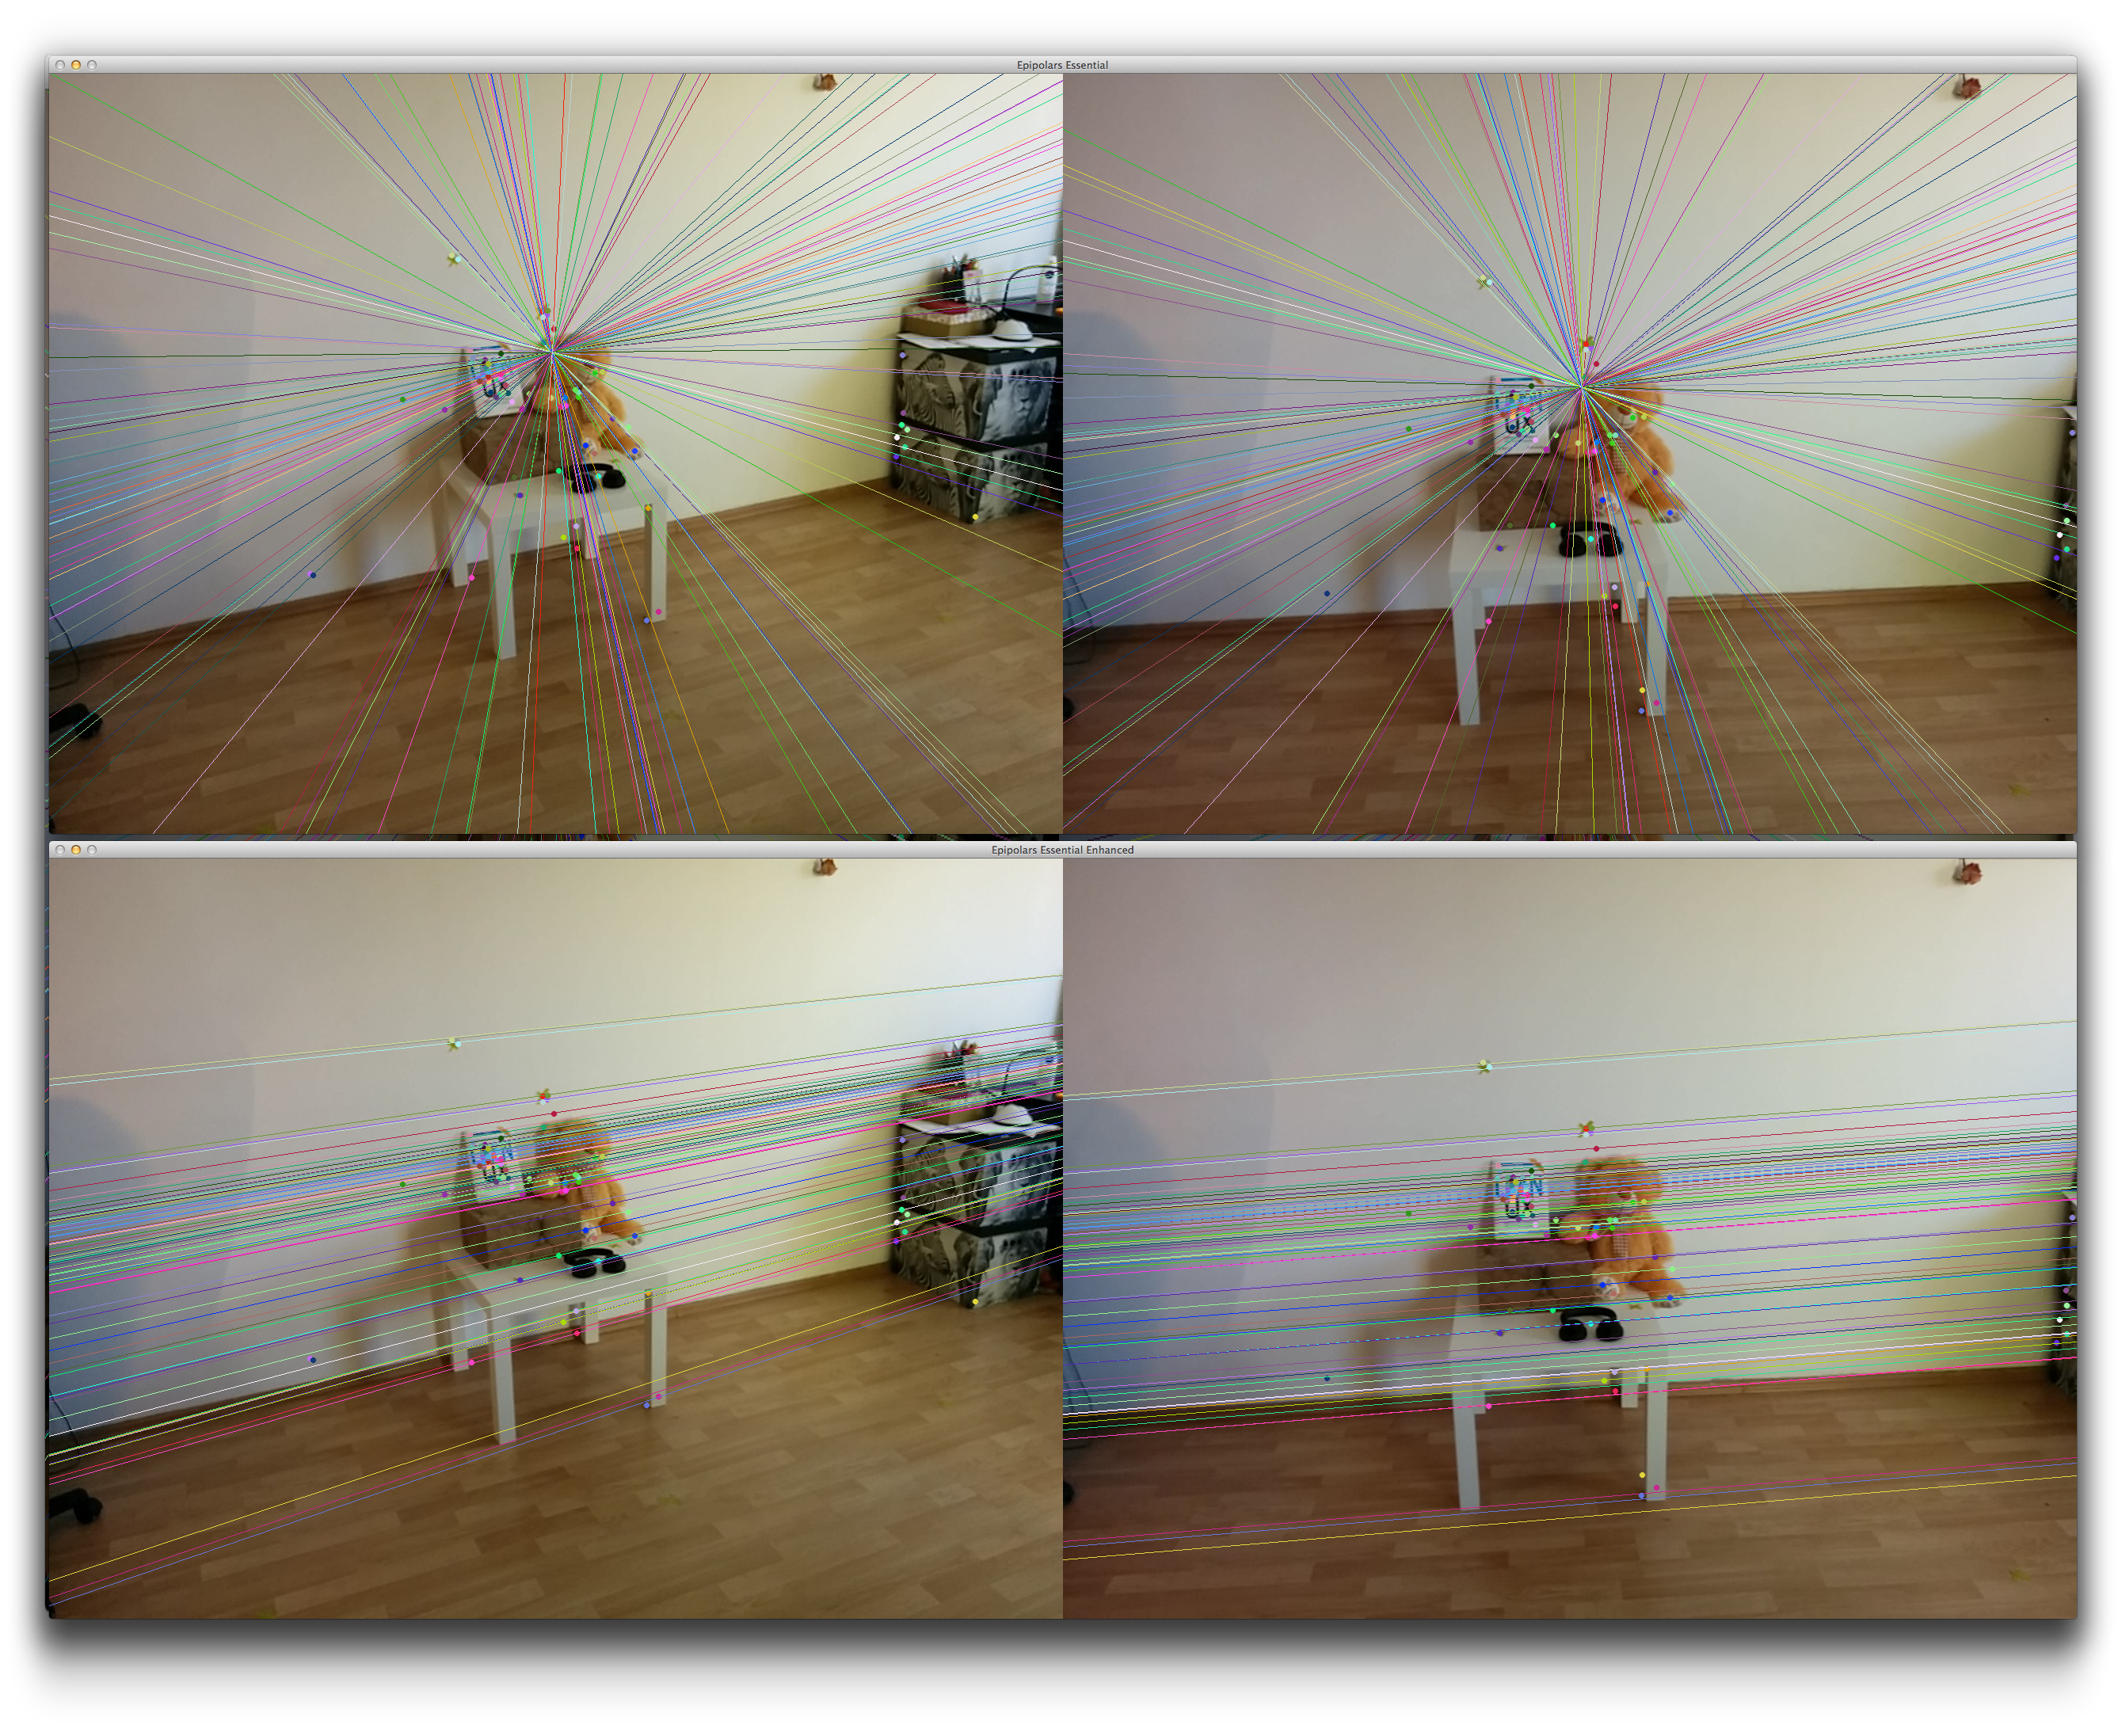
\includegraphics[width=0.8\textwidth]{f_01_5point_comp}
    \caption[Comparison of epipolar lines for 5-point standard and enhanced versions  - 1st example]{Comparison of epipolar lines for 5-point standard and enhanced versions for automatically matched points in images 0.jpg and 1.jpg from test dataset. Some outliers are produced during feature matching process.}
    \label{fig:f_01_5point_comp}
\end{figure}

\begin{figure}[h!]
    \centering
    \includegraphics[width=0.8\textwidth]{f_02_8point_comp}
    \caption[Comparison of epipolar lines for 8-point standard and enhanced versions  - 2nd example]{Comparison of epipolar lines for 8-point standard and enhanced versions for automatically matched points in images 0.jpg and 2.jpg from test dataset. Some outliers are produced during feature matching process.}
    \label{fig:f_02_8point_epi_comp}
\end{figure}

\begin{figure}[h!]
    \centering
    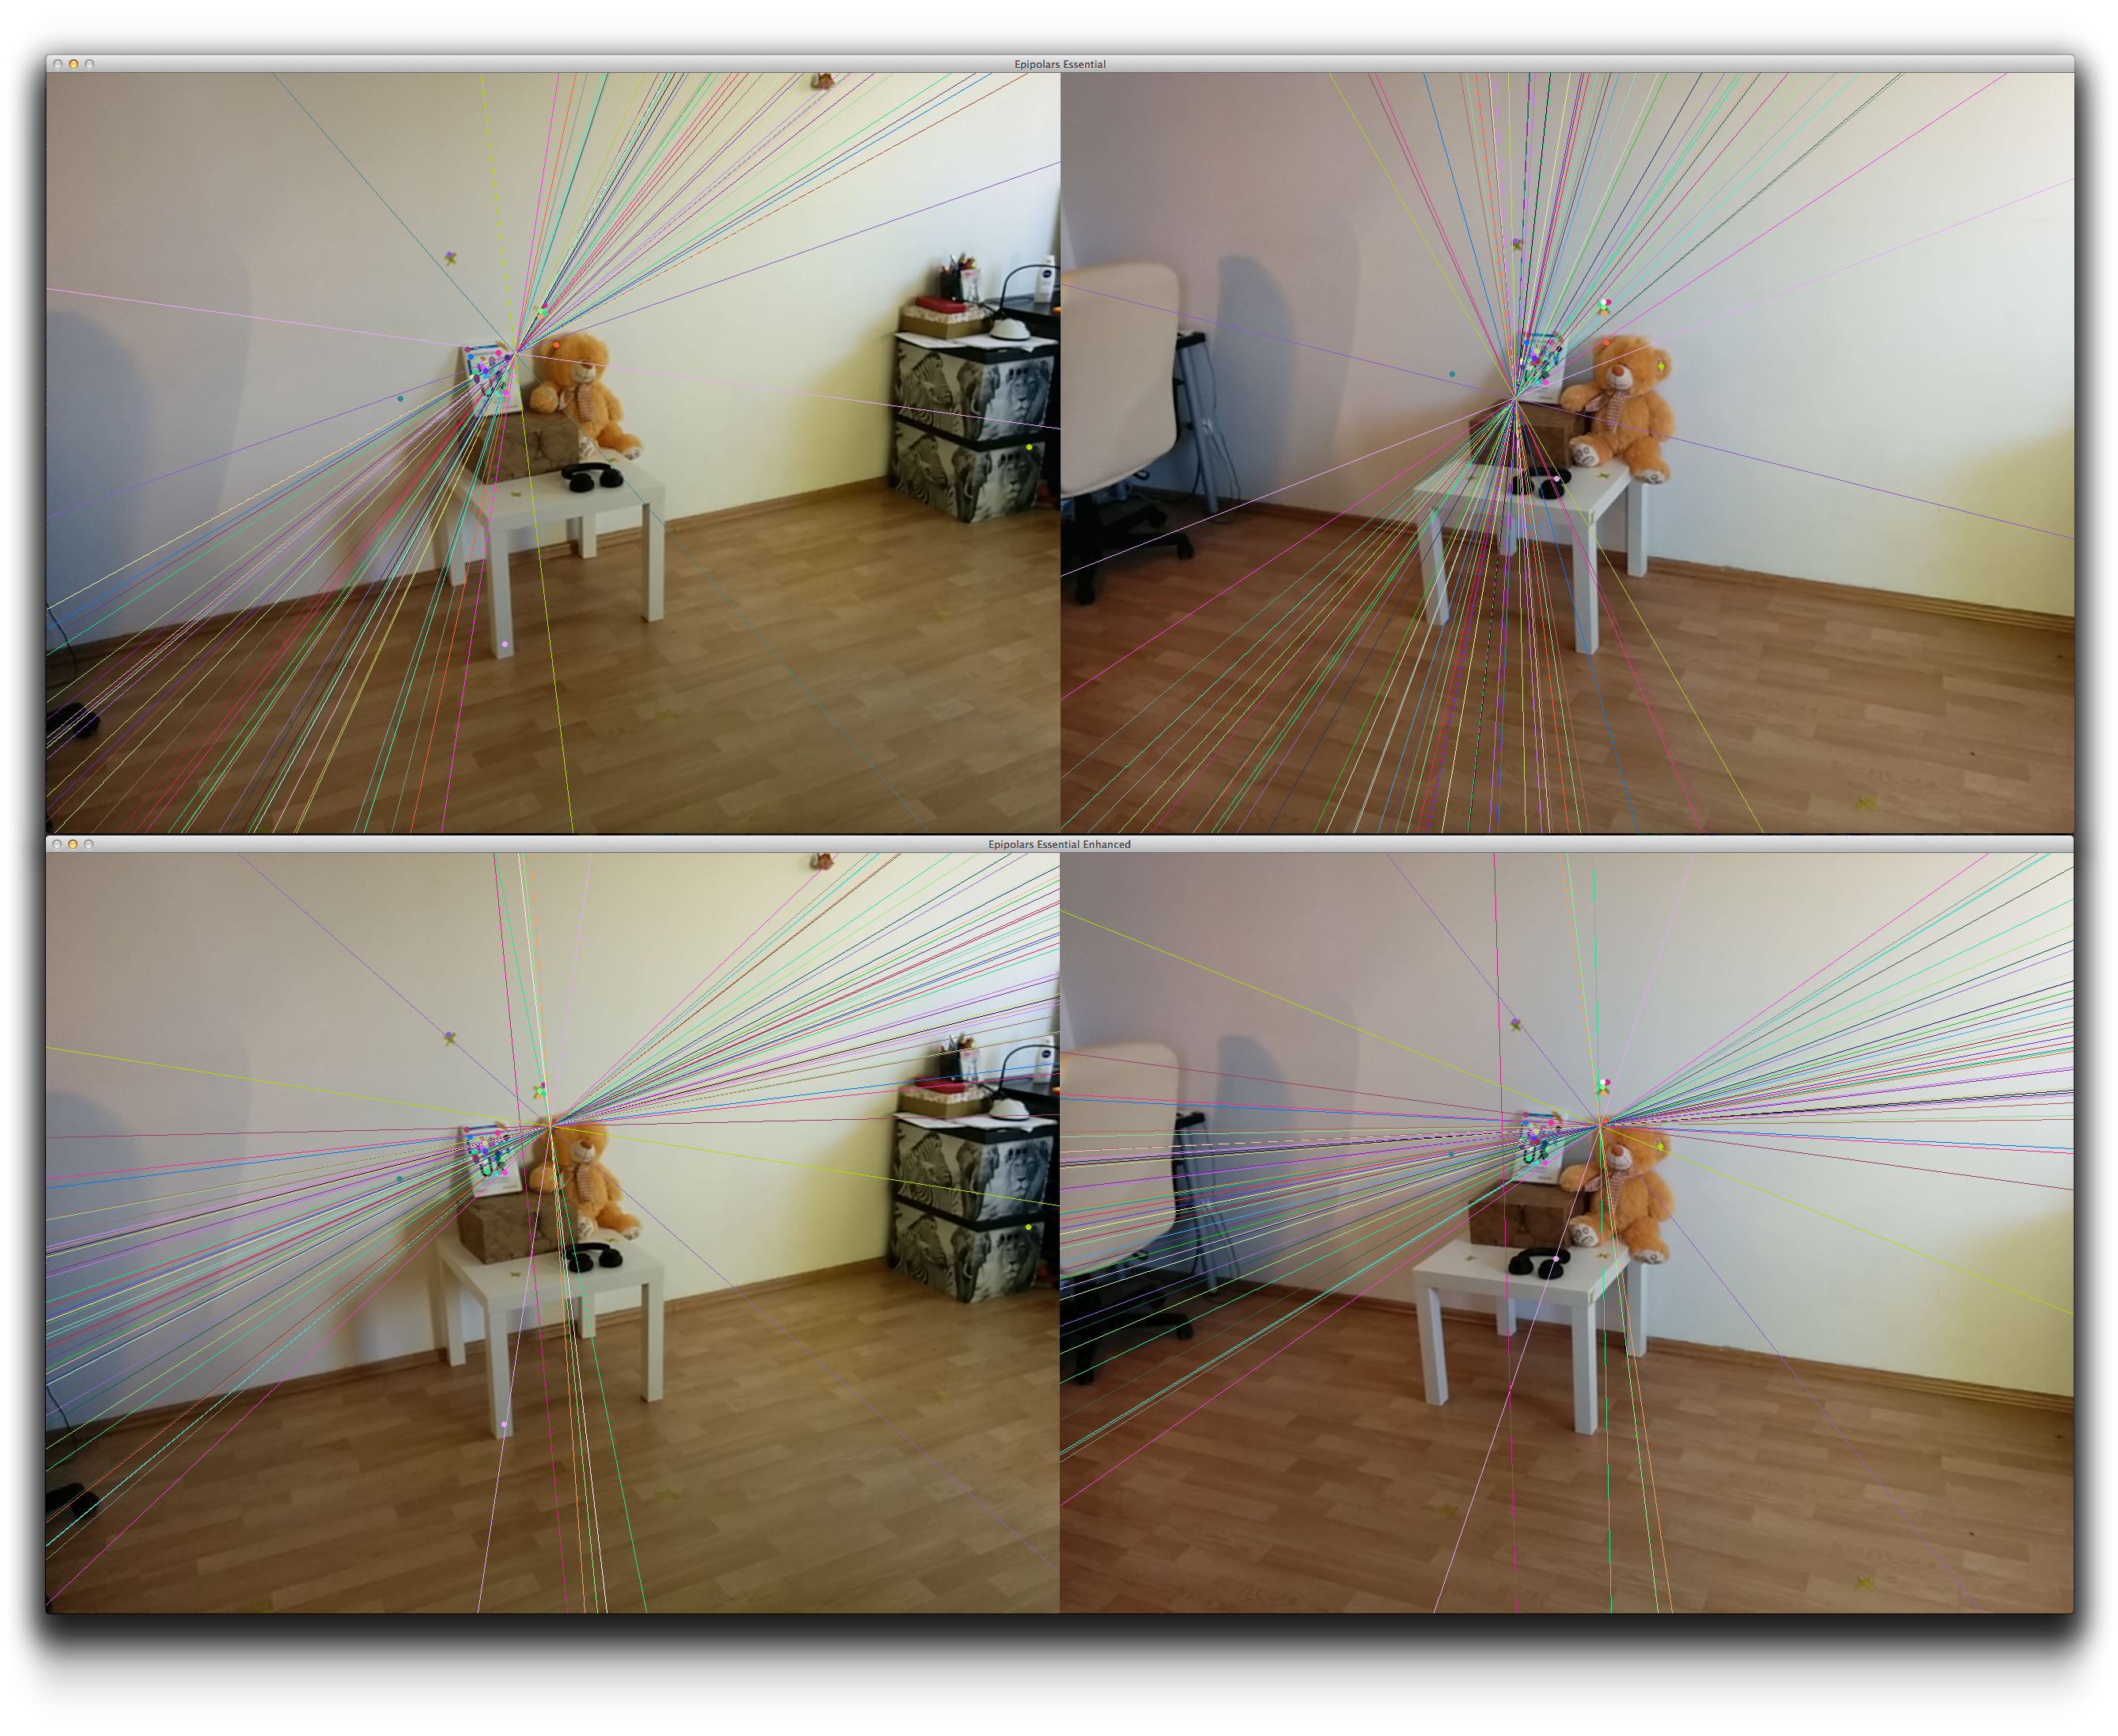
\includegraphics[width=0.8\textwidth]{f_02_5point_comp}
    \caption[Comparison of epipolar lines for 5-point standard and enhanced versions  - 2nd example]{Comparison of epipolar lines for 5-point standard and enhanced versions for automatically matched points in images 0.jpg and 2.jpg from test dataset. Some outliers are produced during feature matching process.}
    \label{fig:f_02_5point_epi_comp}
\end{figure}


